\section{Интеграция пользовательских предпочтений в алгоритм. Декомпозиция по референсным векторам.}
Идея, на первый взгляд ортогональная теме many-objective\\
Соображение 1: нередко мы ограничены в вычислительных возможностях, но
лицо, принимающее решения, может сформулировать свои предпочтения. Если запустить непредвзятый алгоритм, который не отдает предпочтения критериям, то мы ничего не найдём.\\
- Почему бы не интегрировать предпочтения в алгоритм? \\
- Ряд специализированных идей: лексикографическая оптимизация критериев,
большее преимущество решениям-«локтям» (англ. knees, локально наиболее
выпуклые участки Парето-фронта), и т.д.\\
Соображение 2: «если Ваш алгоритм считает себя preference-free, Вы просто
захардкодили свои предпочтения»\\
- Например: «абсолютные/относительные значения критериев имеют смысл». \\
- Crowding distance в алгоритме NSGA-II инвариантна относительно только
линейных преобразований\\
- Максимизация гиперобъема приводит к разным результатам, если
перемасштабировать или преобразовать критерии\\
- Почему бы не признаться в этом честно и не дать пользователю задавать свои
предпочтения явно? :)\\

Декомпозиция по референсным векторам

Выберем множество достаточно разнообразных референсных векторов,
которые покрывали бы желаемый фрагмент Парето-фронта равномерно\\
- Место для явного указания пользовательских предпочтений\\
Будем решать множество однокритериальных задач, по одной для каждого
вектора, давая обмениваться решениями\\
Если повезет, сойдемся вдоль каждого вектора к Парето-фронту

\begin{figure}[!ht]

\begin{center}
    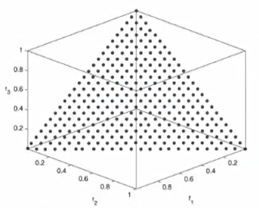
\includegraphics[width=0.3\linewidth]{images/Reference_vector.PNG}
    \caption{Reference vector}
    \label{fig:mpr}
    
\end{center}

\end{figure}
